\usetikzlibrary{arrows.meta,calc,decorations.pathreplacing}

\tikzset{
    simple wire/.style={very thick,>=Latex},
    wire/.style={line width=1.5pt,>=Latex},
    wire small/.style={line width=1pt,>=Latex},
    binLabel/.style={font=\tt},
    hiBox/.style={red, very thick, draw},
    >=Latex,
}

\begin{frame}[fragile,label=constructInstrHW]{multiplying by 16}
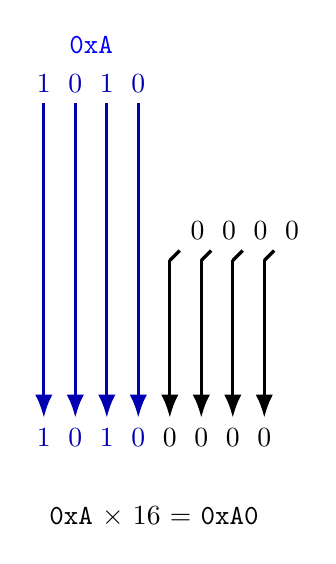
\begin{tikzpicture}
    \foreach \x/\v in {0/1,1/0,2/1,3/0} {
        \draw[simple wire,->,blue!70!black] ($(0, 0) + \x*(0.4, 0)$) node[above] {\v} -- ++(0, -4) node[below] {\v};
    }
    \node[anchor=south,blue] at (0.6, .5) {\tt 0xA};
    \foreach \x in {4,5,6,7} {
        \draw[simple wire,->] ($(0, -2) + \x*(0.4, 0)$) -- ++(0, -2) node[below] {0};
        \draw[simple wire] ($(0, -2) + \x*(0.4, 0)$) -- ++(.125, .125) node[above right] {0};
    }
    \node[anchor=north] at (1.4, -5) {{\tt 0xA} $\times$ 16 = {\tt 0xA0}};
\end{tikzpicture}
\end{frame}

\begin{frame}[fragile,label=shL]{shift left}
\begin{itemize}
    \item ~\xcancel{\tt {\keywordstyle shr} \$-4, \%reg}
    \item instead: {\tt {\keywordstyle shl} \$4, \%reg} (``\textbf{sh}ift \textbf{l}eft'')
    \item ~\xcancel{\tt value >> (-4)}
    \item instead: {\lstinline|value << 4|}
\end{itemize}
\begin{tikzpicture}
\foreach \x/\v in {0/1,1/0,2/1,3/1} {
    \node[anchor=south] at ($(0,0) + \x*(0.4, 0)$) {\tt \v};
}
\foreach \x/\v in {4/0,5/0,6/1,7/0} {
    \node[anchor=south] at ($(0,0) + \x*(0.4, 0)$) {\tt \v};
    \node[anchor=north] at ($(0, -2.5) - 4*(0.4,0) + \x*(0.4, 0)$) {\tt \v};
}
\foreach \x in {4,5,6,7} {
    \draw[simple wire,->] ($(0,0) + \x*(0.4, 0)$) -- ($(0,-2.5) - 4*(0.4, 0) + \x*(0.4, 0)$);
}
\foreach \x in {4,5,6,7} {
    \draw[simple wire,->,alt=<2>{red}{black}] ($(.5, 0) + (0,-2) + \x*(0.4, 0)$) node[above] {\tt 0} -- ($(0,-2.5) + \x*(0.4, 0)$);
    \node[anchor=north,alt=<2>{red}{black}] at ($(0,-2.5) + \x*(0.4, 0)$) {\tt 0};
}
\end{tikzpicture}
\end{frame}

\begin{frame}[fragile,label=shLwires]{shift left}
    \begin{itemize}
    \item x86 instruction: {\keywordstyle shl} --- shift left
    \item {{\keywordstyle shl} \tt\$\textit{amount}, \%reg} (or variable: {\tt{\keywordstyle shl} \%cl, \%reg})
    \end{itemize}
\begin{tikzpicture}
\draw[blue,decorate,decoration=brace,ultra thick] (-.2, .7) -- (13., .7) node[midway, above] {\%reg (initial value)};
\draw[blue,decorate,decoration={brace,mirror},ultra thick] (-.2, -3.1) -- (13., -3.1) node[midway, below] {\%reg (final value)};
\foreach \x/\v in {0/1,1/0,2/1,3/1} {
    \node[anchor=south] at ($(0,0) + \x*(0.4, 0)$) {\tt \v};
}
\foreach \x/\v in {4/0,5/0,6/1,7/\strut\ldots,27/\strut\ldots,28/0,29/1,30/0,31/0} {
    \node[anchor=south] at ($(0,0) + \x*(0.4, 0)$) {\tt \v};
    \node[anchor=north] at ($(0, -2.5) - 4*(0.4,0) + \x*(0.4, 0)$) {\tt \v};
}
\foreach \x in {4,5,6,7,...,31} {
    \draw[simple wire,->] ($(0,0) + \x*(0.4, 0)$) -- ($(0,-2.5) - 4*(0.4, 0) + \x*(0.4, 0)$);
}
\foreach \x in {28,29,30,31} {
    \draw[simple wire,->,alt=<2>{red}{black}] ($(.5, 0) + (0,-2) + \x*(0.4, 0)$) node[above] {\tt 0} -- ($(0,-2.5) + \x*(0.4, 0)$);
    \node[anchor=north,alt=<2>{red}{black}] at ($(0,-2.5) + \x*(0.4, 0)$) {\tt 0};
}
\end{tikzpicture}
\end{frame}

\begin{frame}[fragile,label=leftShift]{left shift in math}
% FIXME: 1s/2s/4s place diagram
\begin{tabular}{l@{\hspace{3cm}}l}
\lstinline|1 << 0 == 1| & \tt 0000 0001 \\
\lstinline|1 << 1 == 2| & \tt 0000 001\color{red!60}0 \\
\lstinline|1 << 2 == 4| & \tt 0000 01\color{red!60}00 \\
~ & ~ \\
\lstinline|10 << 0 == 10| & \tt 0000 1010 \\
\lstinline|10 << 1 == 20| & \tt 0001 010\color{red!60}0 \\
\lstinline|10 << 2 == 40| & \tt 0010 10\color{red!60}00 \\
~ & ~ \\
\lstinline|-10 << 0 == -10| & \tt 1111 0110 \\
\lstinline|-10 << 1 == -20| & \tt 1110 110\color{red!60}0 \\
\lstinline|-10 << 2 == -40| & \tt 1101 10\color{red!60}00 \\
\end{tabular}
\vspace{0.3cm}
\begin{center}
\begin{visibleenv}<2->
\large
$x$ \lstinline|<<| $y = x \times 2^y$
\end{visibleenv}
\end{center}
\end{frame}

